\section*{Summenformeln}

\textbf{Gauss}
\begin{equation}
    \sum_{k=1}^{n} k = \frac{n(n+1)}{2}
\end{equation}

\textbf{Gerade Zahlen}
\begin{equation}
    \sum_{k=1}^{n} 2k = n*(n+1)
\end{equation}

\textbf{Ungerade Zahlen}
\begin{equation}
    \sum_{k=1}^{n} 2*(k-1) = n^2
\end{equation}

\textbf{Quadrat Zahlen}
\begin{equation}
    \sum_{k=1}^{n} k^2 = \frac{n*(n+1)*(2n+1)}{6}
\end{equation}

\textbf{Kubische Zahlen}
\begin{equation}
    \sum_{k=1}^{n} k^3 = (\frac{n*(n+1))}{2})^2
\end{equation}

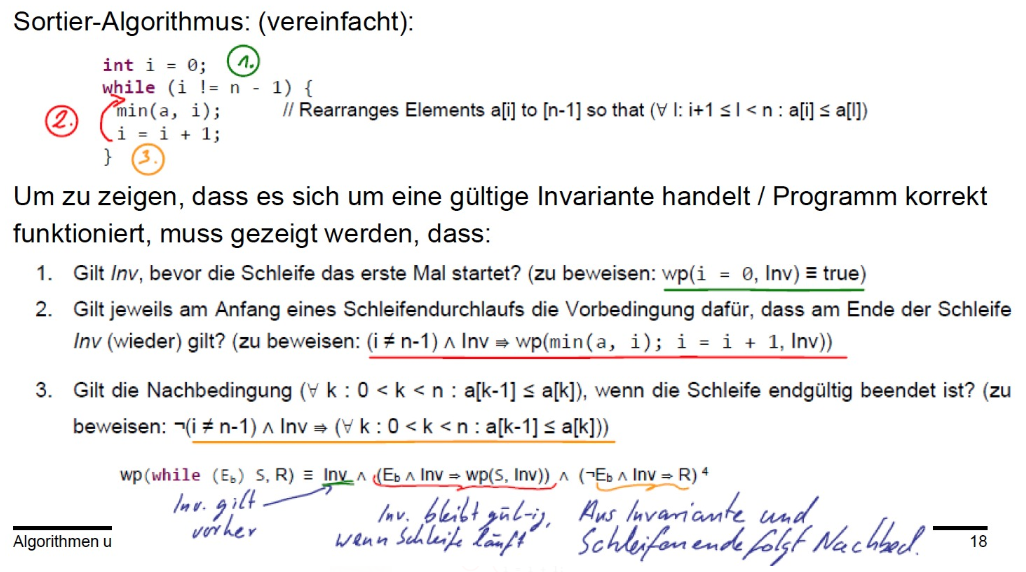
\includegraphics[width=\linewidth]{images/invariante}